\subsubsection{Crossover}
\label{sec:bg:ga:var:cx}
  The variation operator in genetic algorithms often involves a procedure known as \emph{crossover},
  which emulates the process of genetic recombination observed in nature.\footnote{
    This is referred to as \emph{crossing-over} 
    in~\autocite{hollandAdaptationNaturalArtificial1992a}.
  }
  This process involves the exchange of genetic material between two individuals to create a new 
  generation.

  \begin{definition}[Crossover operator]
  \label{def:crossover_operator}
    A crossover operator is a variation operator that is used to create new individuals from 
    existing ones by performing a recombination of their genetic material.

    Formally, it is a variadic function represented as 
    
    \[
      X : \mathbb{P} \times \mathbb{R} \times \cdots \to \mathbb{P};
      (P, \rho, \dots) \mapsto X(P, \rho, \dots)
    \]
    
    where:

    \begin{itemize}
      \item \(\mathbb{P}\) is the set of all possible populations,
      \item \(\mathbb{R}\) is the set of real numbers,
      \item \(P\) is the population to be varied,
      \item \(\rho \in [0, 1]\) is the probability of applying the operator to an individual in the 
        population.
    \end{itemize}

  \end{definition}

  For the problem under consideration, we utilize a simplified form of the \emph{single-point 
  crossover}\footnote{See \vref{sec:keen:operators:crossover:single_point}.} operator. 
  This operator selects the first half of the genes from two parent individuals and generates two 
  new offspring by interchanging these selected genes.
  
  For instance, consider two parent individuals selected via the \emph{roulette wheel} selector 
  described earlier: \(I_1 = 1100\) and \(I_2 = 0001\).
  The single-point crossover operator selects the first half of the genes from each parent, i.e., 11
  from \(I_1\) and 00 from \(I_2\), and produces a pair of new chromosomes with the first half, and 
  produces two new offspring by exchanging these selected parts: \(O_1 = 1101\) and \(O_2 = 0000\) 
  (as illustrated in \vref{fig:genetic_algorithms:variation:crossover:single_point}).

  \begin{figure}[ht!]
    \centering
    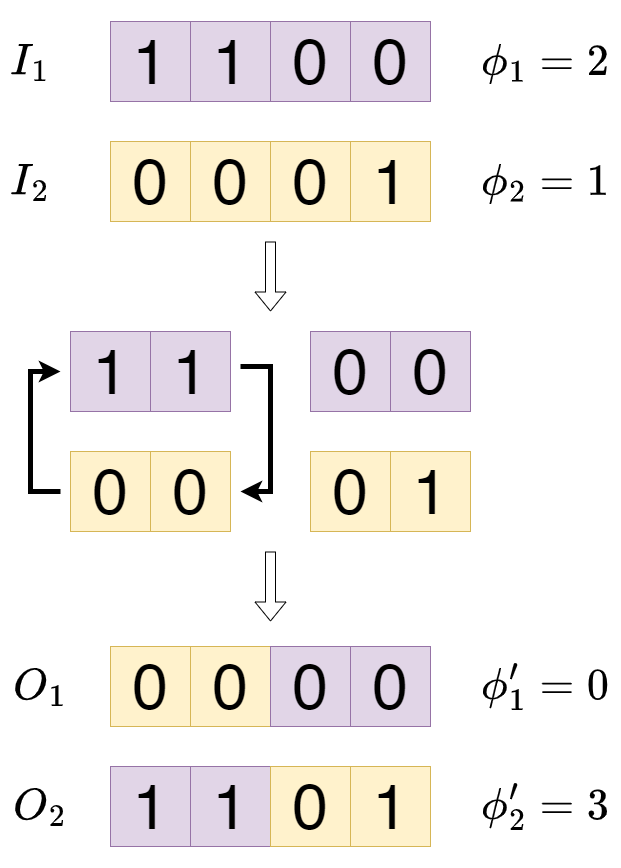
\includegraphics[width=0.3\textwidth]{img/theoretical_framework/Single-Point Crossover.png}
    \caption{Single-point crossover}
    \label{fig:genetic_algorithms:variation:crossover:single_point}
  \end{figure}

  Following another iteration of the single-point crossover operator, we can generate a result as 
  shown in \vref{tab:genetic_algorithms:variation:crossover:single_point}, leading to a new 
  population \(\textbf{O} = \{(0000,\, 0),\, (1101,\, 3),\, (0101,\, 2)\}\).

  \begin{table}[ht!]
    \centering
    \begin{tabular}{|c|c|c|c|}
      \multicolumn{4}{c}{\textbf{Generation 0} \(\to\) \textbf{Generation 1}} \\
      \hline
      \hline
      \(\mathbf{I}\) & \(\Phi_\mathbf{I}\) & \(\mathbf{O}\) & \(\Phi_\mathbf{O}\) \\
      \hline
      \Gape[2pt][2pt]{\(\begin{bmatrix} 1100 \\ 0001 \end{bmatrix}\)}
      & \(\begin{bmatrix} 2 \\ 1 \end{bmatrix}\) 
      & \(\begin{bmatrix} 0000 \\ 1101 \end{bmatrix}\) 
      & \( \begin{bmatrix} 0 \\ 3 \end{bmatrix}\) \\
    \hline
    \(\begin{bmatrix} 0001 \\ 0100 \end{bmatrix}\) 
      & \Gape[2pt][2pt]{\(\begin{bmatrix} 1 \\ 1 \end{bmatrix}\)}
      & \(\begin{bmatrix} 0101 \\ \cdot \end{bmatrix}\)
      & \(\begin{bmatrix} 2 \\ \cdot \end{bmatrix}\) \\[0.5em]
      \hline
    \end{tabular}
    \caption{
      Illustration of the single-point crossover operation. 
      In this procedure, two parent individuals are selected and a cut point is chosen. 
      Each offspring is then formed by combining the genes from the parents: one gets the genes 
      from the first part of the first parent and the second part of the second parent, while the 
      other gets the genes from the first part of the second parent and the second part of the 
      first parent. 
      Here, \(\cdot\) represents a \enquote{discarded} value (since according to the survival 
      rate, only three offspring need to be produced).
    }
    \label{tab:genetic_algorithms:variation:crossover:single_point}
  \end{table}

  If we now use these offspring as-is to create the next generation, we would obtain the
  population shown in \vref{tab:genetic_algorithms:variation:crossover:single_point:2}:

  \begin{table}[ht!]
    \centering
    \begin{tabular}{c | c | c }
      \multicolumn{3}{c}{\textbf{Generation 1}} \\
      \hline
      \hline
      \textbf{Individual} & \textbf{Binary String}  & \textbf{Fitness} \\
      \hline
      \(I_2\)             & \(0001\)                & 1 \\
      \(O_1\)             & \(0000\)                & 0 \\
      \(O_2\)             & \(1101\)                & 3 \\
      \(O_3\)             & \(0101\)                & 2
    \end{tabular}
    \caption{
      Population after applying the single-point crossover operator.
      Note that \(I_2\) is the survivor of the previous generation picked in 
      \vref{sec:background:genetic_algorithms:selection}.
    }
    \label{tab:genetic_algorithms:variation:crossover:single_point:2}
  \end{table}

  \begin{table}[H]
    \centering
    \begin{tabular}{|c|c|c|}
      \hline
            & \textbf{Fitness} & \textbf{Individual}  \\
      \hline
      Best  & 3 & \(O_2\) \\
      Worst & 0 & \(O_1\) \\
      \hline
      \hline
      Average & \multicolumn{2}{c|}{1.25} \\
      \hline
      Standard deviation & \multicolumn{2}{c|}{1.291} \\
      \hline
    \end{tabular}
    \caption{
      Fitness of the population after applying the single-point crossover operator.
      \enquote{Best} refers to the individual with the highest fitness, and \enquote{Worst} refers 
      to the individual with the lowest fitness
    }
    \label{tab:genetic_algorithms:variation:crossover:single_point:fitness}
  \end{table}

  As observed from \vref{tab:genetic_algorithms:variation:crossover:single_point:fitness}, the 
  average fitness of the population has increased from 1 to 1.25, and the fitness of the best 
  individual has improved from 2 to 3. 
  This improvement showcases how the crossover operator helps guide the search towards superior 
  solutions.

  While the crossover operation has indeed enhanced the average fitness of the population, to 
  further augment genetic diversity within the population and prevent premature convergence to 
  suboptimal solutions (local optima), the introduction of a \emph{mutation} operator is often 
  beneficial. 
  This operation will be discussed in the next section.

